% --------------------------------------------------------------------------------

\begin{exercise}

Beweisen Sie die Guldinschen Regeln:

Die Mantelfläche eines um die $z$-Achse rotationssymmetrischen Körpers im $\R^3$ ist gleich der Weglänge die der Schwerpunkt der Kurve die durch den Schnitt der Mantelfläche mit der Halbebene $\Bbraces{(x, y, z) : x > 0, y = 0}$ entsteht bei einer vollen Drehung um die $z$-Achse mal der Weglänge dieser Kurve.

Das Volumen eines um die $z$-Achse rotationssymmetrischen Körpers $K$ im $\R^3$ ist gleich der Weglänge die der Schwerpunkt der Fläche $\Bbraces{(x, y, z) \in K,: x > 0, y = 0}$ bei einer vollen Drehung um die $z$-Achse mal dem Flächenmaß dieser Fläche.

Sie dürfen annehmen, dass diese Schnittkurven als Funktion von $z$ dargestellt werden können, d.h. der Manterl ist $(r(z) \cos \varphi, r(z) \sin \varphi, z)$.

\end{exercise}

% --------------------------------------------------------------------------------

\begin{solution}

\phantom{}

\begin{enumerate}[label = \arabic*.]

    \item Teil:

    Seien $S$ der Schwerpunkt, $M$ die Mantelfläche, und $H$ die Halbebene.
    Sei $r: (a, b) \to \R$ der Radius der $x$-$y$-Kreis-Scheiben des rotationssymmetrischen Körpers $K$, und $a$ und $b$ die maximale bzw. minimale $z$-Koordinate eines Punktes $\in K$.
    Wir parametrisieren den Mantel vermöge
    
    \begin{align*}
        \phi:
            (a, b) \times [0, 2 \pi) \to M,
            (z, \varphi) \mapsto (r(z) \cos \varphi, r(z) \sin \varphi, z),
    \end{align*}
    
    und die Kurven durch
    
    \begin{align*}
        \begin{matrix}
            \gamma_1: & [a, b]     & \to & M \cap H,                      & z & \mapsto & (r(z), 0, z), \\
            \gamma_2: & [0, 2 \pi) & \to & M \cap (\R^2 \times \pr_3(S)), & t & \mapsto & (\pr_1(S) \cos t, \pr_1(S) \sin t, \pr_3(S)).
        \end{matrix}
    \end{align*}
    
    \begin{center}
        \begin{tikzpicture}[scale = 0.5]
    
            \begin{scope}[xshift = -6cm]
    
                \draw [->] (-4, 0) -- (4, 0) node [right] {$x, y$};
                \draw [->] (0, -4) -- (0, 4) node [above] {$z$};
    
                \draw (-2, 0) -- (0, 3) -- (2, 0);
    
                \draw [dashed, xshift = 1pt, yshift = 1pt] ( 0, 3)   -- node [above right] {$\gamma_1$} (2, 0);
                \draw [dashed]                             (-1, 1.5) -- node [below left]  {$\gamma_2$} (1, 1.5);
                
                \draw (0, 0)   circle (1pt) node [below left]  {$a$};
                \draw (0, 3)   circle (1pt) node [above right] {$b$};
                \draw (1, 1.5) circle (1pt) node [below left]  {$S$};
    
            \end{scope}
    
            \begin{scope}[xshift = 6cm]
    
                \draw [->] (-4, 0) -- (4, 0) node [right] {$x$};
                \draw [->] (0, -4) -- (0, 4) node [above] {$y$};
    
                \draw          (0, 0) circle (3cm);
                \draw [dashed] (0, 0) circle (1.5cm);
    
                \draw [dashed, yshift = -1pt] (0, 0) -- (3, 0);
    
                \draw ( 1.5,  0)   circle (1pt) node [above right] {$S$};
                \draw ( 1.5,  0)                node [below right] {$\gamma_1$};
                \draw (-1.5, -1.5)              node               {$\gamma_2$};
    
            \end{scope}
    
        \end{tikzpicture}
    \end{center}
    
    \includegraphicsboxed{Ana1&2/Ana1&2 - 11.1.10 Korollar.png}
    
    Laut Korollar 11.1.10, gilt
    
    \begin{align*}
        \ell(\gamma_1)
        =
        \ell_1(b),
        \quad
        \ell_1(x)
        =
        \ell(\gamma_1 |_\bbraces{a, x})
        =
        \Int[a][x]
        {
            |\gamma_1^\prime(z)|
        }{z}
        =
        \Int[a][x]
        {
            \sqrt{r^\prime(z)^2 + 1}
        }{z}.
    \end{align*}
    
    Laut der Formel für den Kreis-Umfang, gilt
    
    \begin{align*}
        \ell(\gamma_2)
        =
        2 \pi \pr_1(S).
    \end{align*}
    
    \begin{center}
        \begin{tcolorbox}[standard jigsaw, opacityback = 0]
    
          \centering
          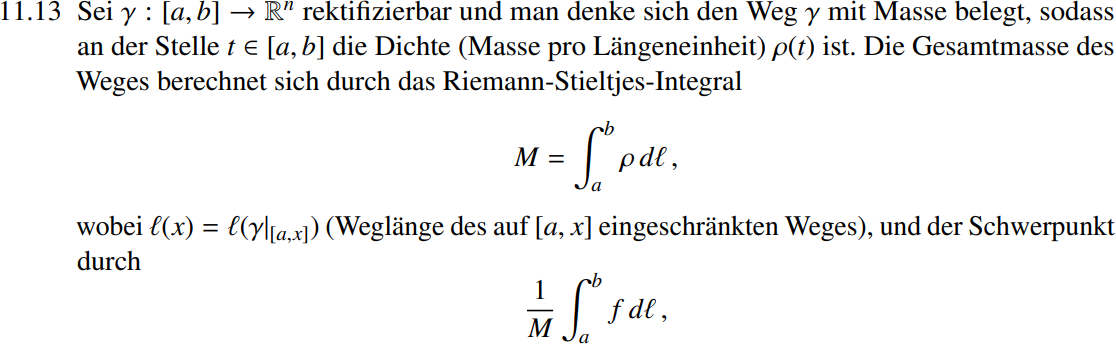
\includegraphics[width = 0.75 \textwidth]{Ana1&2/Ana1&2 - 11.13.1.png} \\
          \vspace{0.25cm}
          \hspace{0.75cm}
          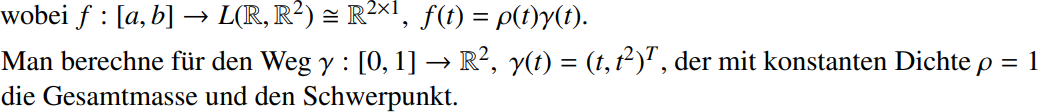
\includegraphics[width = 0.7  \textwidth]{Ana1&2/Ana1&2 - 11.13.2.png}
    
        \end{tcolorbox}
    \end{center}
    
    Wir berechnen den, in 11.13 sauber definierten, Schwerpunkt
    
    \begin{multline*}
        S
        =
        \pbraces
        {
            \Int[a][b]{}{\ell}
        }^{-1}
        \pbraces
        {
            \Int[a][b]{\gamma_1}{\ell}
        }
        =
        \pbraces
        {
            \Int[a][b]
            {
                \ell_1^\prime(z)
            }{z}
        }^{-1}
        \pbraces
        {
            \Int[a][b]
            {
                \gamma_1(z)
                \ell_1^\prime(z)
            }{z}
        } \\
        =
        \ell(\gamma_1)^{-1}
        \pbraces
        {
            \Int[a][b]
            {
                r(z)
                \sqrt{r^\prime(z) + 1}
            }{z},
            0,
            \Int[a][b]
            {
                z
                \sqrt{r^\prime(z) + 1}
            }{z}
        }.
    \end{multline*}
    
    \includegraphicsboxed{Ana1&2/Ana1&2 - 11.2.5 Satz.png}
    
    Dabei haben wir Satz 11.2.5, und den Hauptsatz der Differential- und Integral-Rechnung verwendet.
    
    \includegraphicsboxed{Ana3/Ana3 - Satz 4.2.15.png}
    
    Wir verwenden Satz 4.2.15 und berechnen zu guter Letzt
    
    \begin{align*}
        \mathcal H^2(M)
        =
        2 \pi
        \Int[a][b]
        {
            |r(z)|
            \sqrt{1 + r^\prime(z)^2}
        }{z}
        =
        2 \pi
        \ell(\gamma_1)
        \pr_1(S)
        =
        \ell(\gamma_1)
        \ell(\gamma_2).
    \end{align*}

    \item Teil:
    
    Sei $F = K \cap H$, diese Fläche.
    Wir parametrisieren den Körper mit Zylinderkoordinaten, d.h. vermöge

    \begin{align*}
        \phi:
            \Omega := \Bbraces{(t, \varphi, z): 0 \leq \varphi < 2 \pi, a < z < b, 0 < t < r(z)},
            (t, \varphi, z) \mapsto (t \cos \varphi, t \sin \varphi, z),
    \end{align*}

    und diese Fläche durch

    \begin{align*}
        \psi:
            B := \Bbraces{(x, z) \in \R^3: a < z < b, 0 < x < r(z)} \to F,
            (x, z) \mapsto (x, 0, z).
    \end{align*}

    Wir definieren den (neuen), nirgendwo sauber definierten, Schwerpunkt

    \begin{align*}
        S
        :=
        \pbraces
        {
            \Int[F]{}{\mathcal H^2}
        }^{-1}
        \pbraces
        {
            \Int[F]{\id}{\mathcal H^2}
        },
    \end{align*}

    und berechnen dessen $1$-te Komponente

    \begin{multline*}
        \pr_1(S)
        =
        \frac{1}{\mathcal H^2(F)}
        \Int[\psi(B)]
        {
            \pr_1 \circ \id
        }{\mathcal H^2}
        =
        \frac{1}{\mathcal H^2(F)}
        \Int[B]
        {
            (\pr_1 \circ \id)(\psi(x, z))
            \vbraces
            {
                \derivative[][\psi]{x}
                \times
                \derivative[][\psi]{z}
            }
        }{(x, z)} \\
        =
        \frac{1}{\mathcal H^2(F)}
        \Int[B]
        {
            x
            \underbrace{|e_1 \times e_3|}_1
        }{(x, z)}
        =
        \frac{1}{\mathcal H^2(F)}
        \Int[a][b]
        {
            \Int[0][r(z)]
            {
                x
            }{x}
        }{z}
        =
        \frac{1}{\mathcal H^2(F)}
        \frac{1}{2}
        \Int[a][b]
        {
            r(z)^2
        }{z}.
    \end{multline*}

    Dabei haben wir Satz 4.2.14 verwendet.

    \includegraphicsboxed{Ana3/Ana3 - Satz 4.2.14.png}

    Wir verwenden die Transformationsformel und berechnen zu guter Letzt

    \begin{multline*}
        \lambda^3(K)
        =
        \Int[\phi(\Omega)]{}{\lambda^3}
        \stackrel
        {
            \text{TRAFO}
        }{=}
        \Int[\Omega]{t}{(t, \varphi, z)}
        =
        2 \pi
        \Int[a][b]
        {
            \Int[0][r(z)]
            {
                t
            }{t}
        }{z} \\
        =
        2 \pi
        \frac{1}{2}
        \Int[a][b]
        {
            r(z)^2
        }{z}
        =
        2 \pi
        \mathcal H^2(F) \pr_1(S)
        =
        \ell(\gamma_2) \mathcal H^2(F).
    \end{multline*}

\end{enumerate}

\end{solution}

% --------------------------------------------------------------------------------
